\subsection{Giảm chiều dữ liệu với phương pháp PCA (Principal Component Analysis)}
\paragraph{}{\textbf{Phân tích thành phần chính} (Principal Component Analysis - PCA) \cite{mlcoban-pca} là phương pháp giảm chiều dữ liệu bằng cách tìm một hệ tọa độ mới sao cho:}

\begin{itemize}
    \item Các thành phần chính (Principal Components - PCs) là các hướng có phương sai lớn nhất.
    \item Các PCs vuông góc (trực giao) với nhau.
    \item  PC1 mang nhiều thông tin nhất, PC2 mang thông tin còn lại.
\end{itemize}

\subsubsection{Các bước thực hiện PCA}
\label{label: pca}

\paragraph{}{Tính vector kỳ vọng của toàn bộ dữ liệu:}
\[
\bar{x} = \frac{1}{N} \sum_{n=1}^{N} x_n
\]
\paragraph{}{Tính độ lệch chuẩn của từng đặc trưng:}
    \[
    \sigma_d = \sqrt{\frac{1}{N} \sum_{n=1}^{N} (x_{n,d} - \bar{x}_d)^2}
    \]
    trong đó:
    \begin{itemize}
        \item \( x_{n,d} \) là giá trị của đặc trưng thứ \( d \) tại điểm dữ liệu \( n \).
        \item \( \bar{x}_d \) là giá trị trung bình của đặc trưng \( d \).
        \item \( \sigma_d \) là độ lệch chuẩn của đặc trưng \( d \).
    \end{itemize}

\paragraph{}{Trừ mỗi điểm dữ liệu đi vector kỳ vọng của toàn bộ dữ liệu:}
\[
\hat{x}_n = x_n - \bar{x}
\]
\paragraph{}{Nếu các đặc trưng không có cùng miền giá trị thì ta chuẩn hóa bằng phương pháp Z-Score (xem \ref{label:standart scaler})}
\[
\hat{x}_n = \frac{x_n - \bar{x}}{\sigma_d}
\]
\paragraph{}{Tính ma trận hiệp phương sai:}
\[
S = \frac{1}{N} \hat{X} \hat{X}^T
\]

\paragraph{}{Tính các trị riêng và vector riêng có norm bằng 1 của ma trận này, sắp xếp chúng theo thứ tự giảm dần của trị riêng.}

\paragraph{}{Chọn \( K \) vector riêng với \( K \) trị riêng lớn nhất để xây dựng ma trận \( U_K \) có các cột tạo thành một hệ trực giao. \( K \) vectors này, còn được gọi là các thành phần chính, tạo thành một không gian con gần với dữ liệu ban đầu đã chuẩn hóa.}

\paragraph{}{Chiếu dữ liệu ban đầu đã chuẩn hóa \( \hat{X} \) xuống không gian con tìm được:}
\[
Z = U_K^T \hat{X}
\]

\paragraph{}{Dữ liệu mới chính là tọa độ của các điểm dữ liệu trên không gian mới.}

\paragraph{}{Dữ liệu ban đầu có thể tính được xấp xỉ theo dữ liệu mới như sau:}
\[
x \approx U_K Z + \bar{x}
\]


\begin{figure}[H]
    \centering
    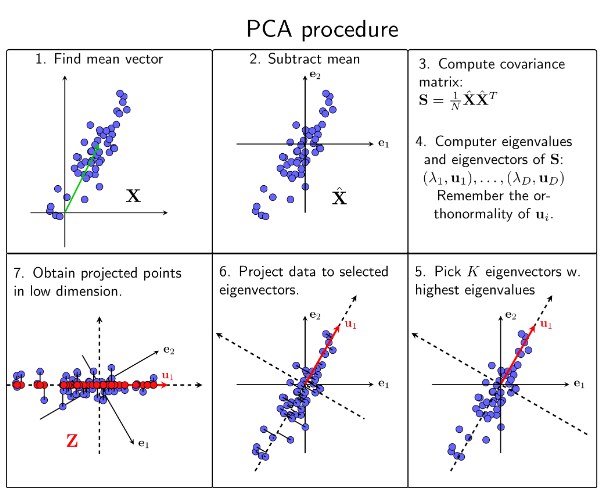
\includegraphics[width=0.7\textwidth]{img/mathPCA.png}
    \caption{Minh họa các bước thực hiện PCA}
    \label{fig:PCA_steps}
\end{figure}





\subsubsection{Ví dụ PCA từ ma trận 2 chiều về 1 chiều}

Giả sử ta có ma trận 4X2 

\[
X =
\begin{bmatrix}
2 & 3 \\
3 & 5 \\
5 & 8 \\
7 & 10
\end{bmatrix}
\]

\paragraph{}{\textbf{Chuẩn hóa dữ liệu}}

Tính trung bình từng cột:

\[
\mu_1 = \frac{2+3+5+7}{4} = 4.25, \quad \mu_2 = \frac{3+5+8+10}{4} = 6.5
\]

Khi đó, ta có:

\[
X' = X - \mu
\]

\[
X' =
\begin{bmatrix}
-2.25 & -3.5 \\
-1.25 & -1.5 \\
0.75 & 1.5 \\
2.75 & 3.5
\end{bmatrix}
\]

\paragraph{}\textbf{Tính ma trận hiệp phương sai}

\[
S  =
\begin{bmatrix}
4.9167 & 6.8333 \\
6.833 & 9.6667
\end{bmatrix}
\]


\paragraph{}\textbf{Tính trị riêng và véc tơ riêng}

Giải phương trình trị riêng:

\[
\begin{vmatrix}
4.9167 - \lambda &6.8333  \\
6.833  & 9.6667 - \lambda
\end{vmatrix} = 0
\]

Giải phương trình bậc hai, ta được:

\[
\lambda_1 = 14.5259648 , \quad \lambda_2 = 0.0573
\]

Véc tơ riêng tương ứng:

\[
v_1 =
\begin{bmatrix}
-0.815\\ 0.579
\end{bmatrix}, \quad
v_2 =
\begin{bmatrix}
-0.579\\ -0.815
\end{bmatrix}
\]

\paragraph{}\textbf{Chiếu dữ liệu và trục chính}

\[
Z = X' V_1 =
\begin{bmatrix}
-2.25 & -3.5 \\
-1.25 & -1.5 \\
0.75 & 1.5 \\
2.75 & 3.5
\end{bmatrix}
\begin{bmatrix} -0.815\\ 0.579 \end{bmatrix}
=
\begin{bmatrix}
-4.156 \\
-1.946 \\
1.657 \\
4.446
\end{bmatrix}
\]

Vậy, ma trận 4x2 chiều đã được chuyển thành ma trận 4x1 chiều với giá trị mới \( Z \).
